\documentclass{beamer}
%
% Choose how your presentation looks.
%
% For more themes, color themes and font themes, see:
% http://deic.uab.es/~iblanes/beamer_gallery/index_by_theme.html
%
\mode<presentation>
{
  \usetheme{default}      % or try Darmstadt, Madrid, Warsaw, ...
  \usecolortheme{default} % or try albatross, beaver, crane, ...
  \usefonttheme{default}  % or try serif, structurebold, ...
  \setbeamertemplate{navigation symbols}{}
  \setbeamertemplate{caption}[numbered]
}

\usepackage[english]{babel}
\usepackage[utf8x]{inputenc}

\usepackage{amstext}
%\usepackage{coloremoji}
\usepackage{layout}
\usepackage{multirow}

\usepackage{graphicx}
\graphicspath{ {figs/} }

\setbeameroption{hide notes}
\setbeamertemplate{note page}[plain]
\usepackage{listings}
\usepackage{datetime}
\usepackage{url}

% specifications for presenter mode
%\beamerdefaultoverlayspecification{<+->}
%\setbeamercovered{transparent}

% math shorthand
\usepackage{bm}
\usepackage{amsmath}
\usepackage{mathtools}
\newcommand{\D}{\mathcal{D}}
\newcommand{\E}{\mathbb{E}}
\newcommand{\F}{\mathcal{F}}
\newcommand{\X}{\mathcal{X}}
\newcommand{\lik}{\mathcal{L}}
\DeclarePairedDelimiterX{\infdivx}[2]{(}{)}{%
  #1\;\delimsize\|\;#2%
}
\newcommand{\infdiv}{D\infdivx}
\DeclarePairedDelimiter{\norm}{\lVert}{\rVert}
\DeclareMathOperator*{\argmin}{arg\,min}
\DeclareMathOperator*{\argmax}{arg\,max}

% Bibliography
\usepackage{natbib}
\bibpunct{(}{)}{,}{a}{}{;}
\usepackage{bibentry}

%\nobibliography*
\title[zinbwave-droplasso]{Differential Expression Analysis Techniques for
  Single-Cell RNA-seq Experiments}
\subtitle{\vspace*{0.5em} \scriptsize for the Computational Biology Doctoral
  Seminar (CMPBIO 293),\\ organized by N.~Yosef \& T.~Ashuach, Spring 2018, UC
  Berkeley}
\author{Kevin Benac and Nima Hejazi}
\institute{Group in Biostatistics,\\ University of California, Berkeley}
\date{11 April 2018}

%%%%%%%%%%%%%%%%%%%%%%%%%%%%%%%%%%%%%%%%%%%%%%%%%%%%%%%%%%%%%%%%%%%%%%%%%%%%%%%%

%\setcounter{tocdepth}[2]
\AtBeginSubsection[]{
\begin{frame}{Outline}
\tableofcontents[currentsection,currentsubsection]
\end{frame}
}

%%%%%%%%%%%%%%%%%%%%%%%%%%%%%%%%%%%%%%%%%%%%%%%%%%%%%%%%%%%%%%%%%%%%%%%%%%%%%%%%

\begin{document}

\begin{frame}
  \titlepage
\end{frame}

%%%%%%%%%%%%%%%%%%%%%%%%%%%%%%%%%%%%%%%%%%%%%%%%%%%%%%%%%%%%%%%%%%%%%%%%%%%%%%%%
\section{Introduction}
\subsection{Data}
%%%%%%%%%%%%%%%%%%%%%%%%%%%%%%%%%%%%%%%%%%%%%%%%%%%%%%%%%%%%%%%%%%%%%%%%%%%%%%%%

\begin{frame}{The Data: Single-Cell RNA-seq}
\begin{itemize}
  \itemsep10pt
  \item scRNA-seq fast growing approach to measure the genome-wide transcriptome of many individual cells in parallel (Kolodziejczyk et al., 2015).
  \item Major advance compared to standard “bulk” RNA sequencing to investigate complex heterogeneous tissues,
  \item Access to cell-to-cell variability: better accuracy.
\end{itemize}

\end{frame}

%%%%%%%%%%%%%%%%%%%%%%%%%%%%%%%%%%%%%%%%%%%%%%%%%%%%%%%%%%%%%%%%%%%%%%%%%%%%%%%%

\begin{frame}{The Data: Single-Cell RNA-seq}

%No free lunch thm
\begin{itemize}
  \itemsep10pt
  \item However, analysis of scRNA-seq data challenging.
  \item In one cell, only a tiny amount of RNA is present and large fraction of polyadenylated RNA can be stochastically lost during sample preparation steps (cell lysis, reverse transcription or amplification). \\
 $ \Longrightarrow$ Many genes fail to be detected although they are expressed!
  \item In practice, not uncommon to end up with a matrix of read counts where about 80\% of the coefficients are zeros.
  \item This zeros are called \textit{dropouts}.
\end{itemize}

\end{frame}

%%%%%%%%%%%%%%%%%%%%%%%%%%%%%%%%%%%%%%%%%%%%%%%%%%%%%%%%%%%%%%%%%%%%%%%%%%%%%%%%

\begin{frame}{The Data: Single-Cell RNA-seq}

\begin{table}[ht]
\centering
\begin{tabular}{rrrrrrrrrrr}
  \hline
 & Cell1 & Cell 2 & Cell 3 & Cell 4 & Cell 5 & Cell 6 & Cell 7  \\ 
  \hline
Xkr4 & 0 & 0 & 0 & 14 & 0 & 0 & 0  \\ 
  Syt11 & 1 & 9 & 2 & 2 & 0 & 0 & 0  \\ 
  Cpe & 0 & 0 & 16 & 0 & 0 & 0 & 0  \\ 
  Rp1 & 0 & 0 & 0 & 0 & 0 & 0 & 0  \\ 
  Gm73 & 0 & 0 & 0 & 0 & 0 & 0 & 0  \\ 
  Gm79 & 0 & 0 & 0 & 0 & 0 & 0 & 0  \\ 
  Mpl15 & 8 & 8 & 6 & 1 & 0 & 0 & 0  \\ 
  Gm61 & 0 & 0 & 0 & 0 & 0 & 3 & 0 \\ 
  Lypla1 & 1 & 23 & 266 & 1 & 0 & 1 & 0 \\ 
  Tcea1 & 63 & 101 & 18 & 29 & 2 & 34 & 0  \\ 
   \hline
\end{tabular}
\end{table}

\end{frame}

\begin{frame}{The Data: Single-Cell RNA-seq}

\begin{itemize}
  \itemsep10pt
  \item Raises modelling and computational issues.
  \item Need to detect a signal when most of the values are zeros only because they are missing.
  \item Traditional methods used for bulk RNA-seq data might not  be sensible anymore.
\end{itemize}

\end{frame}

%%%%%%%%%%%%%%%%%%%%%%%%%%%%%%%%%%%%%%%%%%%%%%%%%%%%%%%%%%%%%%%%%%%%%%%%%%%%%%%%
\subsection{Objective}
%%%%%%%%%%%%%%%%%%%%%%%%%%%%%%%%%%%%%%%%%%%%%%%%%%%%%%%%%%%%%%%%%%%%%%%%%%%%%%%%

\begin{frame}{The Objective: Differential Expression}

\begin{itemize}
  \itemsep10pt
  \item ...
\end{itemize}

\end{frame}

%%%%%%%%%%%%%%%%%%%%%%%%%%%%%%%%%%%%%%%%%%%%%%%%%%%%%%%%%%%%%%%%%%%%%%%%%%%%%%%%

\begin{frame}{The Objective: Differential Expression}

\begin{itemize}
  \itemsep10pt
  \item ...
\end{itemize}

\end{frame}

%%%%%%%%%%%%%%%%%%%%%%%%%%%%%%%%%%%%%%%%%%%%%%%%%%%%%%%%%%%%%%%%%%%%%%%%%%%%%%%%

\begin{frame}{The Objective: Differential Expression}

\begin{itemize}
  \itemsep10pt
  \item ...
\end{itemize}

\end{frame}

%%%%%%%%%%%%%%%%%%%%%%%%%%%%%%%%%%%%%%%%%%%%%%%%%%%%%%%%%%%%%%%%%%%%%%%%%%%%%%%%
\section{Methodology}
\subsection{ZINB-WaVE}
%%%%%%%%%%%%%%%%%%%%%%%%%%%%%%%%%%%%%%%%%%%%%%%%%%%%%%%%%%%%%%%%%%%%%%%%%%%%%%%%

\begin{frame}{ZINB-WaVE}

\begin{itemize}
  \itemsep10pt
  \item Method that leads to low-dimensional representations of the data the same way PCA or tSNE does. \pause
  \item However accounts for zero inflation (dropouts), over-dispersion, and the count nature of the data.
  \item No need for normalization.
\end{itemize}

\end{frame}
%%%%%%%%%%%%%%%%%%%%%%%%%%%%%%%%%%%%%%%%%%%%%%%%%%%%%%%%%%%%%%%%%%%%%%%%%%%%%%%%




\begin{frame}{ZINB-WaVE}
Mathematical set-up:
\begin{itemize}
  \itemsep10pt
  \item $n$ samples (single-cells),
  \item $J$ genes,
  \item $Y_{ij}$ read counts for gene $j$ in cell $i$, $1\leq \ldots \leq n, \quad 1\leq j \leq J.$,
  \item $\pi_{ij}$: probability of dropout,
  \item $\mu$: mean expression level.
\end{itemize}

\end{frame}

%%%%%%%%%%%%%%%%%%%%%%%%%%%%%%%%%%%%%%%%%%%%%%%%%%%%%%%%%%%%%%%%%%%%%%%%%%%%%%%%



\begin{frame}{ZINB-WaVE}
\begin{figure}
  \centering
      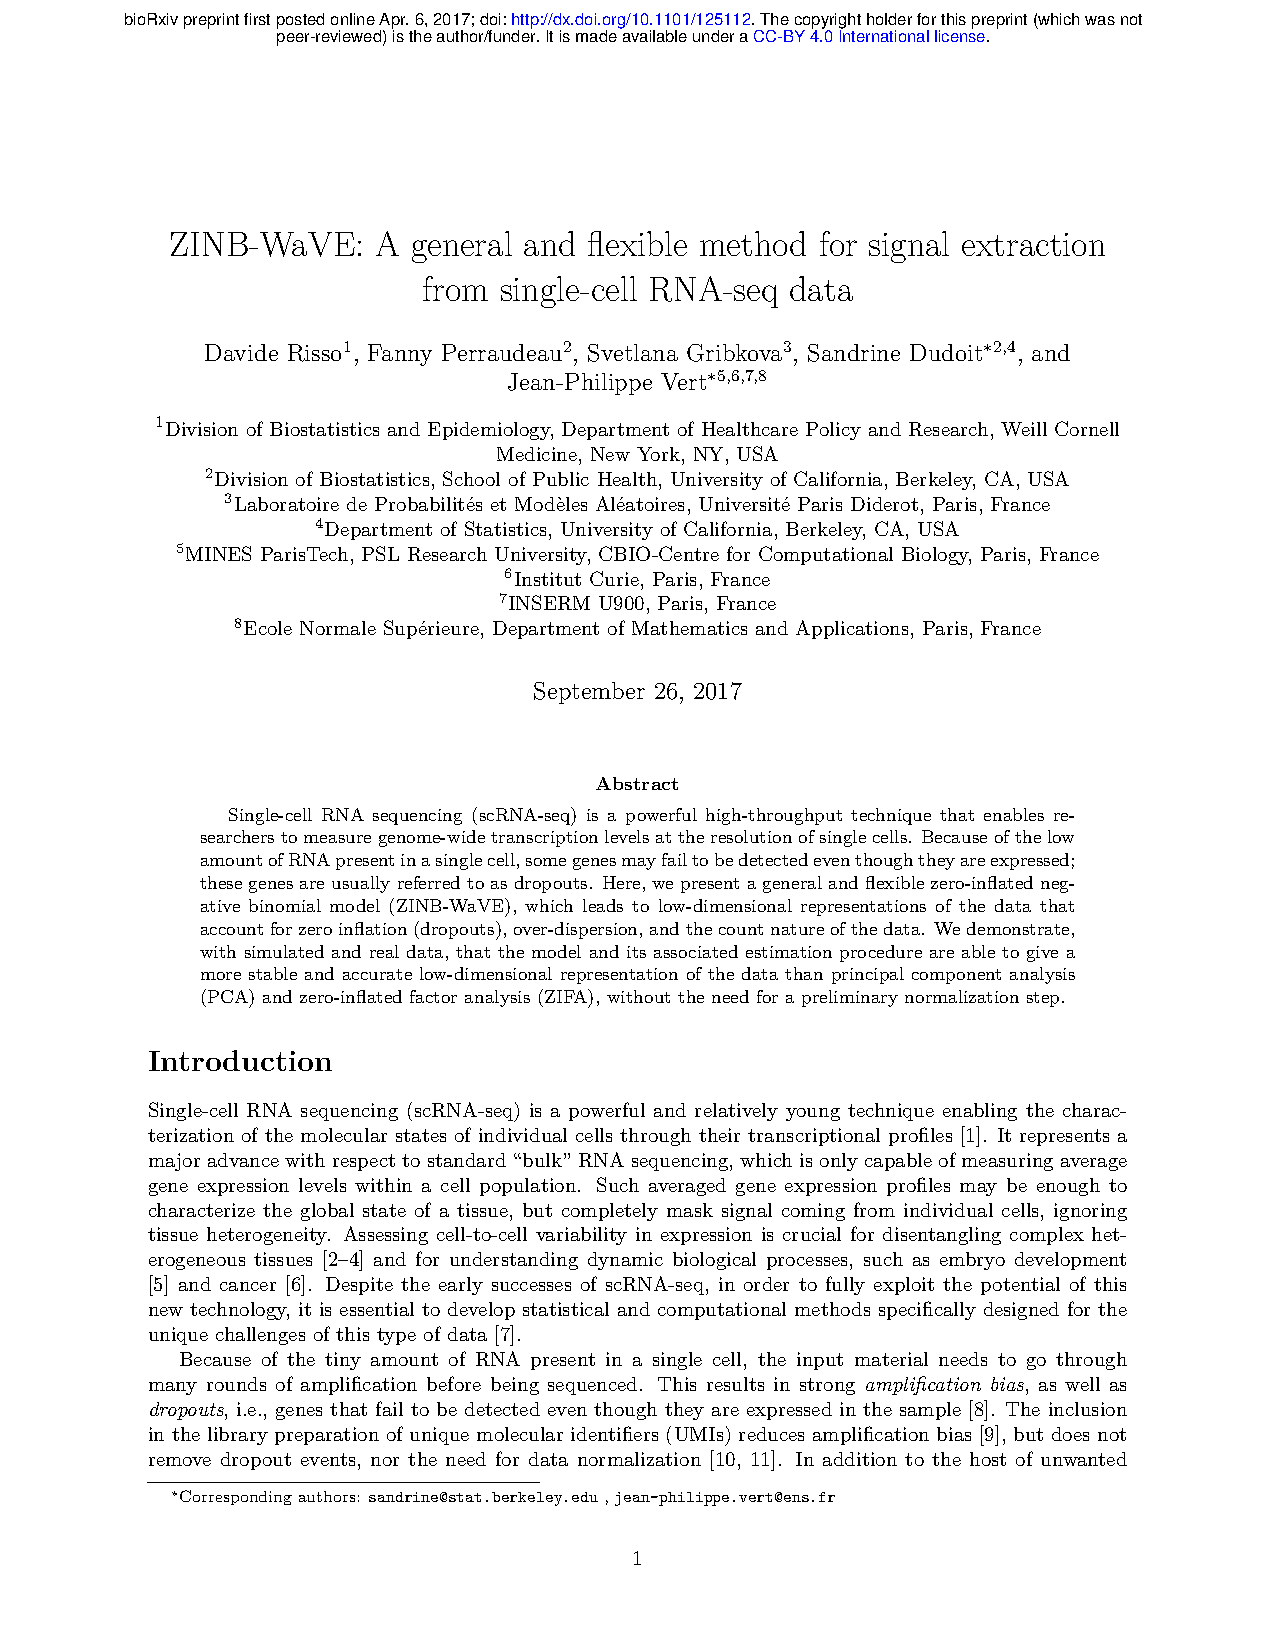
\includegraphics[height=0.5\textheight]{zinbwave}
      \caption{The ZINB-WaVE model}
\end{figure}
\end{frame}

\begin{frame}{ZINB-WaVE}

\begin{itemize}
  \itemsep10pt
  \item ZINB-WaVE mainly used for normalization and dimensionality reduction but can also be used for DE analysis.
  \item Compute weights from the estimated $\pi$ using Bayes formula.
  \item If the observed counts are positive, $w = 1$, otherwise, $0<w<1$.
  \item The higher $\pi$, the lower $w$
\end{itemize}

\end{frame}

%%%%%%%%%%%%%%%%%%%%%%%%%%%%%%%%%%%%%%%%%%%%%%%%%%%%%%%%%%%%%%%%%%%%%%%%%%%%%%%%

\begin{frame}{ZINB-WaVE}

\begin{itemize}
  \itemsep10pt
  \item Once we have the weights, fit a negative binomial glm using the weights.
  \item End-up with a matrix of fitted values.
  \item Not sparse anymore, look more like bulk RNA-seq data.\\
  $\Longrightarrow$ We can use classical tools for differential expression analysis (ex. edgeR or DESeq2 packages in R).
\end{itemize}

\end{frame}

%%%%%%%%%%%%%%%%%%%%%%%%%%%%%%%%%%%%%%%%%%%%%%%%%%%%%%%%%%%%%%%%%%%%%%%%%%%%%%%%
%%%%%%%%%%%%%%%%%%%%%%%%%%%%%%%%%%%%%%%%%%%%%%%%%%%%%%%%%%%%%%%%%%%%%%%%%%%%%%%%
\subsection{DropLasso (Nima)}
%%%%%%%%%%%%%%%%%%%%%%%%%%%%%%%%%%%%%%%%%%%%%%%%%%%%%%%%%%%%%%%%%%%%%%%%%%%%%%%%

\begin{frame}{DropLasso I}

\begin{itemize}
  \itemsep10pt
  \item ...
  \item ...
\end{itemize}

\end{frame}

%%%%%%%%%%%%%%%%%%%%%%%%%%%%%%%%%%%%%%%%%%%%%%%%%%%%%%%%%%%%%%%%%%%%%%%%%%%%%%%%

\begin{frame}{DropLasso II}

\begin{itemize}
  \itemsep10pt
  \item ...
  \item ...
\end{itemize}

\end{frame}

%%%%%%%%%%%%%%%%%%%%%%%%%%%%%%%%%%%%%%%%%%%%%%%%%%%%%%%%%%%%%%%%%%%%%%%%%%%%%%%%

\begin{frame}{DropLasso III}

\begin{itemize}
  \itemsep10pt
  \item ...
  \item ...
\end{itemize}

\end{frame}

%%%%%%%%%%%%%%%%%%%%%%%%%%%%%%%%%%%%%%%%%%%%%%%%%%%%%%%%%%%%%%%%%%%%%%%%%%%%%%%%

\begin{frame}{DropLasso IV}

\begin{itemize}
  \itemsep10pt
  \item ...
  \item ...
\end{itemize}

\end{frame}

%%%%%%%%%%%%%%%%%%%%%%%%%%%%%%%%%%%%%%%%%%%%%%%%%%%%%%%%%%%%%%%%%%%%%%%%%%%%%%%%

\begin{frame}{DropLasso V}

\begin{itemize}
  \itemsep10pt
  \item ...
  \item ...
\end{itemize}

\end{frame}

%%%%%%%%%%%%%%%%%%%%%%%%%%%%%%%%%%%%%%%%%%%%%%%%%%%%%%%%%%%%%%%%%%%%%%%%%%%%%%%%
\subsection{Comparison}
%%%%%%%%%%%%%%%%%%%%%%%%%%%%%%%%%%%%%%%%%%%%%%%%%%%%%%%%%%%%%%%%%%%%%%%%%%%%%%%%

\begin{frame}{ZINB-WaVE v.~DropLasso I}

\begin{itemize}
  \itemsep10pt
  \item ...
  \item ...
\end{itemize}

\end{frame}

%%%%%%%%%%%%%%%%%%%%%%%%%%%%%%%%%%%%%%%%%%%%%%%%%%%%%%%%%%%%%%%%%%%%%%%%%%%%%%%%

\begin{frame}{ZINB-WaVE v.~DropLasso II}

\begin{itemize}
  \itemsep10pt
  \item ...
  \item ...
\end{itemize}

\end{frame}

%%%%%%%%%%%%%%%%%%%%%%%%%%%%%%%%%%%%%%%%%%%%%%%%%%%%%%%%%%%%%%%%%%%%%%%%%%%%%%%%

\begin{frame}{ZINB-WaVE v.~DropLasso III}

\begin{itemize}
  \itemsep10pt
  \item ...
  \item ...
\end{itemize}

\end{frame}

%%%%%%%%%%%%%%%%%%%%%%%%%%%%%%%%%%%%%%%%%%%%%%%%%%%%%%%%%%%%%%%%%%%%%%%%%%%%%%%%
\section{Conclusions}
\subsection{Review}
%%%%%%%%%%%%%%%%%%%%%%%%%%%%%%%%%%%%%%%%%%%%%%%%%%%%%%%%%%%%%%%%%%%%%%%%%%%%%%%%

\begin{frame}{Review}

\begin{itemize}
  \itemsep10pt
  \item ...
  \item ...
\end{itemize}

\end{frame}

%%%%%%%%%%%%%%%%%%%%%%%%%%%%%%%%%%%%%%%%%%%%%%%%%%%%%%%%%%%%%%%%%%%%%%%%%%%%%%%%

% don't want dimming with references
\setbeamercovered{}
\beamerdefaultoverlayspecification{}

\begin{frame}[c,allowframebreaks]{References}

\small
\bibliographystyle{plainnat}
\nocite{*}
\bibliography{refs}
\itemize

\end{frame}

%%%%%%%%%%%%%%%%%%%%%%%%%%%%%%%%%%%%%%%%%%%%%%%%%%%%%%%%%%%%%%%%%%%%%%%%%%%%%%%%

\end{document}

